\chapter{Diskussion}
% Der Wortakzents tendiert dazu an den Worträndern zu liegen \textit{demarcative property} \cite[S.~144]{Kager1999}.

%- Welche Ergebnisse wurden erzielt?

%- Welche Einschränkungen wurden gemacht? 

%- Wie verfälschen ggfs. die gemachten Einschränken/Annahmen das Ergebnis?
%- Diskusion der Möglichkeit von Overfitting.

%- Vergleich zu ähnlichen Arbeiten ziehen, Unterschiede evaluieren.

%- Diskussion einiger Theorien der Metrischen Phonologie unter dem Licht dieser Arbeit.

%- Lieber alle Features oder nur eine Auswahl? Mehr Features = Besser?

%- Was sind die Vor- und Nachteile in meinem Anwendungsfall der Algorithmen?
%NN erfasst nichtlinearitäten
%JRip sehr gut interprätier- und auswertbar, jedoch logisch redundant teilweise (length < 3 \&\& length=1)
%J48 sehr schnell, gut zum Experimentieren
\section{Generelles}
\label{generelles}

\begin{figure}[h]
    \centering
    \caption{Erkennungsraten aller Featuresets in Prozent.\\
    Jeder Boxplot enthält die Ergebnisse der Testdaten für 2 bis 7 Silbige Wörter. Die schwarze Linie stellt den Median dar, die maximale Länge der Whiskers beträgt 1.5 IQR.}
    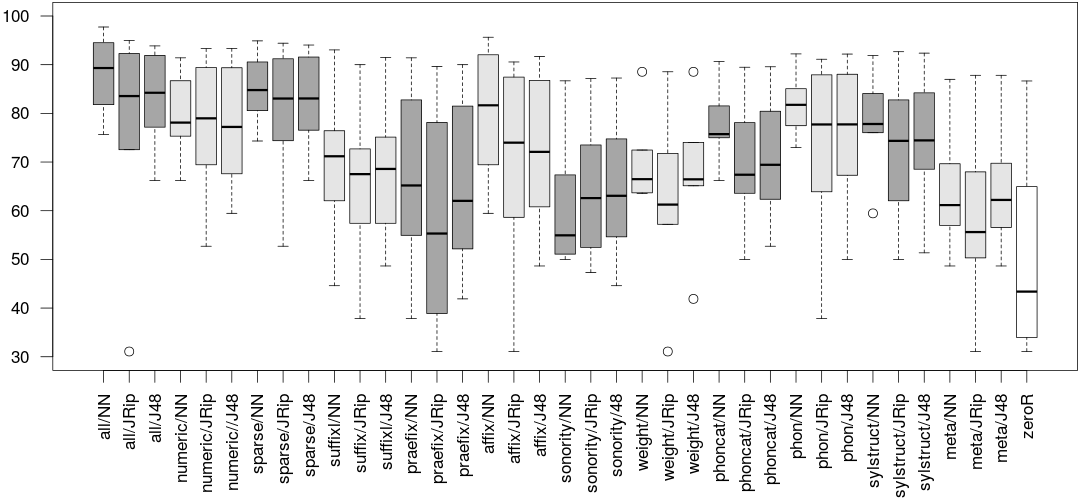
\includegraphics[width=\columnwidth]{figures/featuresets/all.png}
    \label{figure:featuresets_all}
\end{figure}
Die Varianz der Ergebnisse der Featuresets über die Modelle hinweg (Abbildung \ref{figure:featuresets_all}) ist interessant, da eine kleine Varainz eine größere Unabhängigkeit der Regeln von der Silbenanzahl vermuten lässt. Liefert ein Modell über alle Silbenzahlen hinweg ähnliche Ergebnisse, kann man vermuten, dass die Features eine größere Allgemeingültigkeit besitzen bzw. in der Regelhierarchie weiter oben stehen. Das praefix-Featureset besitzt eine sehr große Varianz und teilweise sehr gute Ergebnisse. Die weight-Featuresets erzielen durchweg eher mittelmäßige Ergebnisse, aber dies bei sehr geringer Varianz. Eine Vermutung wäre nun, dass gewisse Praefix-Regeln unter bestimmten Bedingungen andere überschreiben, Regeln des Silbengewichts jedoch deutlich allgemeiner und grundlegender sind. phon/NN und sylstruct/NN besitzen auch beide eine sehr kleine Varianz. Da die Features aus phon sehr nahe der phonetische Repräsentation sind, sind diese sehr Grundlegend.
Die Qualität eines grundlegenden Featuressets kann man auch nach der Invarianz gegenüber der Silbenzahl bei möglichst hoher Abstraktion von der phonetischen Repräsentation beurteilen. Beispielsweise besitzt das phon/NN-Modell eine sehr kleine Varianz und liefert gute Ergebnisse, ist jedoch recht nah der direkten phonetischen Repräsentation. Im Gegensatz dazu besitzen die Modelle des weight-Featuresets zwar keine guten Erkennungsraten, jedoch auch eine sehr kleine Varianz. Das Silbengewicht ist dabei ein sehr abstraktes Maß. Durch dieses Qualitätsmaß lassen sich somit Hinweise finden, wie gut linguistische Konzepte verallgemeinerbar sind. In diesem Kontext scheinen praefix und sonority für sich genommen keine gutes Konzepte zu sein.
Wie wir später sehen werden, sind jedoch grade diese beiden Features in Kombination mit anderen sehr gute Regeln möglich. Als einziges Qualitätsmaß ist die Invarianz gegenüber der Silbenzahl daher wohl nicht ausreichend.


\subsection{Die Ergebnisse im Kontext der Korpusgröße und Schwierigkeit der Klassifikation}
\begin{figure}[hb]
    \centering
    \caption{Erkennungsrate je Testset. Differenz der besten Modelle (dunkelgrau) zu ZeroR (hellgrau). Die Breite der Barplots ist proportional zur Anzahl der enthaltenen Wörter.}
    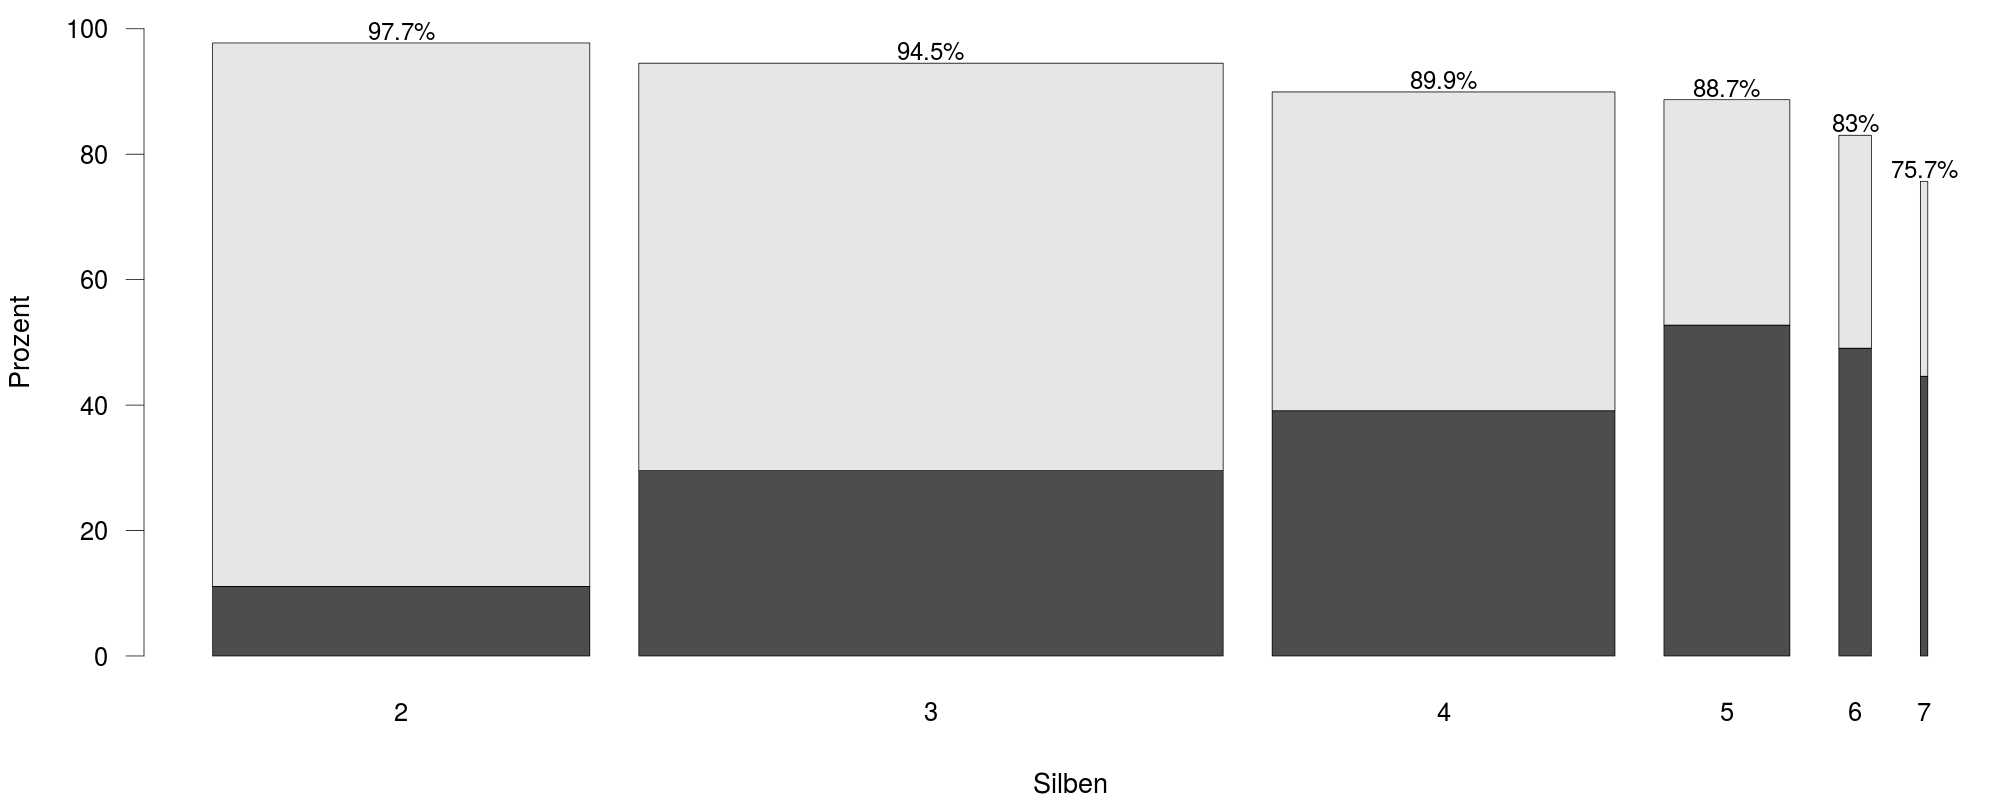
\includegraphics[width=.75\columnwidth]{figures/performance_by_syllables.png}
    \label{figure:results_proportional}
\end{figure}

Wie gut sind meine Ergebnisse wirklich? In Abbildung \ref{figure:results_proportional} sieht man die Differenz des besten Ergebnisses zu ZeroR. Man sieht die positiven Einflüsse der größeren Trainingsmenge sowie das mit zunehmender Silbenanzahl schwieriger werdende Klassifizierungsproblem. Bis fünf Silben wird mit jeder weiteren Silbe ZeroR um etwa ein Viertel schlechter. Sobald alle fünf möglichen Betonungsklassen tatsächlich möglich sind, also die Wörter fünf oder mehr Silben besitzen, liegt ZeroR mehr oder minder konstant bei 30-35\% (siehe Anhang \ref{performance_details}).

\begin{table}[h]
\centering
\caption{Anzahl an Wörter je Trainingsset mit von der häufigsten Klasse abweichender Betonung (gerundet).}
\label{table:wertvolle_woerter}
\begin{tabular}{|ccc|}\hline
{\bf Silben} & {\bf \enquote{wertvolle} Wörter} & {\bf Prozent} \\\hline
2            & 1000                     & 13.3\%   \\
3            & 4000                     & 34.3\%   \\
4            & 3400                     & 49,7\%   \\
5            & 1600                     & 63.7\%   \\
6            & 400                      & 61.2\%   \\
7            & 100                      & 67.6\%   \\\hline
\end{tabular}
\end{table}
Anders gesehen gibt die dunkelgraue Fläche die Anzahl an Wörtern an, die von der häufigsten Klasse abweichen, die also einen höheren Informationsgehalt haben, als die der häufigsten Klasse. So gibt es bei Drei- und Viersilbern die meisten wertvollen Worte, rund viermal so viele wie bei den Zweisilbern (Tabelle \ref{table:wertvolle_woerter}). In diesem Licht ist das Ergebnis der Zweisilber von 97.4\% wahrscheinlich nicht so gut wie es mit den gegebenen Features sein könnte. Mit zunehmender Silbenzahl wird zwar die Klassifizierung schiweriger, jedoch ist der Umfang der Trainingsdaten auch höher, so dass Drei-, Vier- und Fünfsilber trotz des jeweils 1/4 schweren Problems nur geringfügig schlechter sind. Insbesondere bei Fünfsilbern merkt man den Wert von Wörtern mit hohen Informationsgehalt. Obwohl die Gesamtgröße des Trainingssets der Fünfsilber nur ein Drittel so groß ist wie das der Zweisilber, enthält es 40\% mehr wertvolle Wörter. Obwohl das Klassifizierungsproblem doppelt so schwierig ist wie bei Zweisilbern, erreiche ich auf den Fünfsilbern ein nur 9\% schlechteres Ergebnis. Bei den Sechs- und Siebensilbern erkennt man die Auswirkungen der zu kleinen Trainingssets, die Ergebnisse werden verglichen mit den Fünsilbern deutlich schlechter, obwohl das Klassifizierungsproblem etwa gleich schwierig bleibt. Versuchsweise habe ich die Trainings- und Testsets der Fünfsilber dem Umfang der Sechssilber angepasst, um zu sehen, ob man die Beobachtung reproduzieren kann. Tatsächlich erhalte ich statt 88.7\% auf \texttt{all/NN} nun 82.6\% - auf Sechssilbern waren es 83\%. Daraus schlussfolgere ich, dass bei Wörtern mit 5-7 Silben die Lernkurve sehr ähnlich ist.

\subsection{Ergebnisunterschiede auf den \texttt{affix}-Modellen}

Besonderes Augenmerk verdienen die Ergebnisse der \texttt{affix}-Modelle. \texttt{affix/NN} erreicht 89.7\%, während das selbe Featureset in Kombination mit JRip und J48 über 6\% schlechter ist. Woher rührt dieser große Unterschied? Wahrscheinlich kommt er daher, dass jede Regel/jedes Blatt mindestens 20 Wörter enthalten muss. Solch eine Einschränkung gibt es bei den Neuronalen Netzen nicht, sodass jeder noch so seltene Wert eines Feature berücksicht werden kann. Aber lernt das NN nicht einfach nur die Worte auswendig? Immerhin werden unter anderem die führenden und die letzten fünf Phoneme direkt als Features übergeben. Heißt dass, alle Wörter mit weniger als 11 Phonemen werden direkt dem NN übergeben, meist also das gesamte Wort? Nein, denn seltene Werte werden aus den Features gelöscht, so dass ausschließlch die 20 bis 100 häufigsten als Features verwendet werden (Details siehe Anhang \ref{attr_counts}). So ist es möglich häufige Wortanfänge/-enden genau zu differenzieren, und seltenere durch ein Feature mit höherem Abstraktionsgrad (\texttt{prae-/suffix\_phoncat}) auch mit zu erfassen. Da die Wortbetonungen neigt an den Worträndern zu liegen, reicht es offensichtlich beinahe aus, ausschließlich diese bei der Akzentzuweisung zu betrachten. Vielleicht lernen die NN jedoch auch gewisse nichtlineare Korrelationen zwischen Affixen, die den beiden linearen Lernverfahren natürlich verborgen bleiben. Nichts desto trotz haben sich die Affixe als aussagekräftigstes Featureset herausgestellt, von den drei höheren Featuresets abgesehen. Durch Einbeziehung aller weiteren verfügbarer Features in \texttt{all/NN} wird das Ergebnis lediglich um 3.6\% verbessert.

\subsection{Mehr Features, bessere Ergebnisse?}
\label{features_performance_dependancy}
\begin{figure}[h]
    \centering
    \caption{Ergebnisse der Modelle im Verhältnis zur Größe des Featuresets. Bestes Modell je Testset ist hervorgehoben.}
    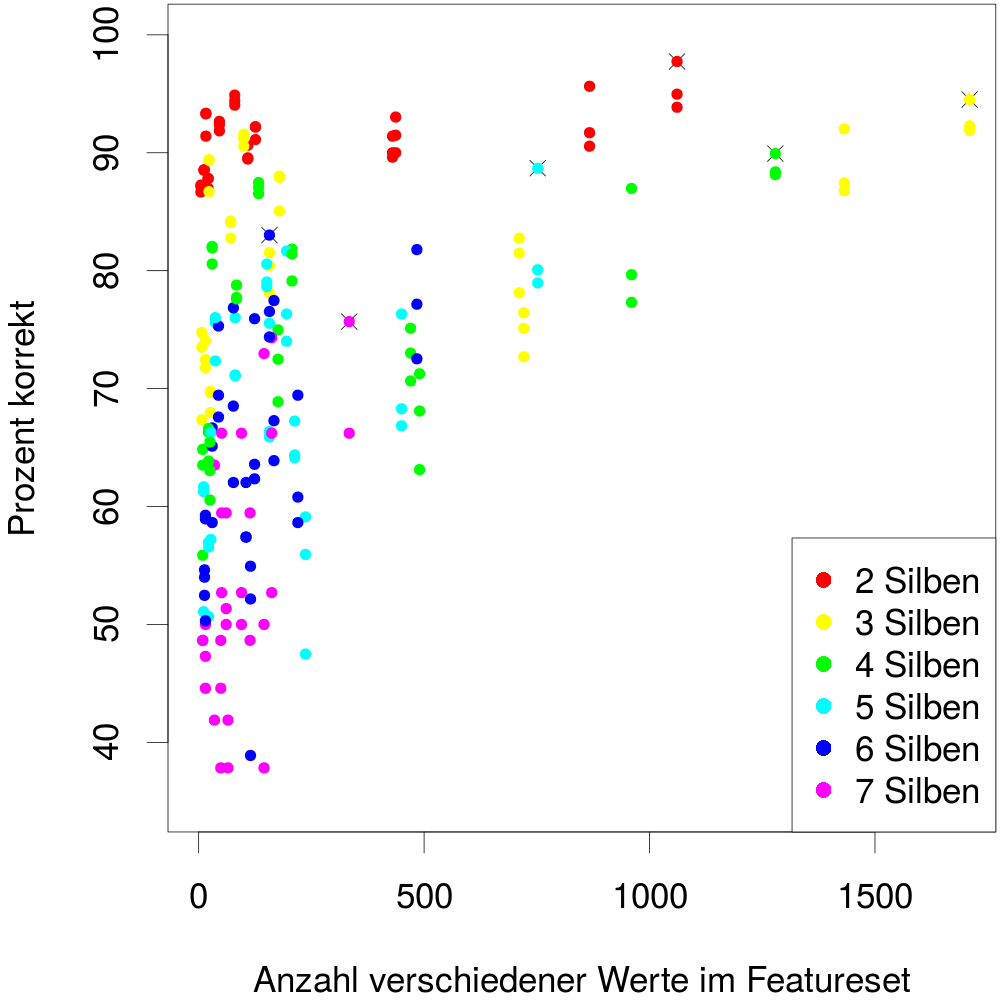
\includegraphics[width=.5\columnwidth]{figures/counts_vs_performance.png}
    \label{figure:counts_vs_performance}
\end{figure}
Den Begriff \enquote{Features} habe ich in der bisherigen Arbeit als \textit{Sammlung} von Merkmalen verwendet. So ist ein beispielsweise \enquote{Hat Suffix \textit{-en}?} ein  Merkmal und \enquote{Hat Suffix \textit{-heit}} ein weiteres. Beide subsumiere ich unter dem Feature \texttt{suffix}, obwohl es eigentlich viele verschiedene Flags sind, ob ein Merkmal vorhanden ist. Wenn ich im Folgenden über die \textit{Merkmalsanzahl} von Feature(sets) spreche, meine ich damit die Gesamtanzahl an Flags für Merkmale von Features. Diese Zahl entspricht im Übrigen der Zahl der Input-Neuronen in Neuronalen Netzen. Numerische Werte zählen ich dabei als ein Wert, da meinen symbolischen Lernverfahren lediglich größer und kleiner unterscheiden und in NN dafür lediglich ein Neuron benötigt wird. Die genaue Zahl der Merkmale je Feature, Featureset und Silbenzahl findet sich in Anhang \ref{attr_counts}

Bis auf eine Ausnahme sind für alle Testsets die Topergebnisse mit dem Featureset erreicht worden, dass die größte Merkmalsanzahl hat (Anhang \ref{performance_details}). Ist es möglich, dass durch die teils sehr große Anzahl an Merkmalen so viele kleine Korrelationen aufsummiert wurden, bis ein gutes Ergebnis erzielt wird? So würde zwar das Modell unter Umständen gut generalisieren, hätte jedoch lediglich statistische Kleinigkeiten zu einem Großen zusammengefügt. Somit wäre man weit von den Kausalzusammenhängen entfernt und tut im Kern dasselbe wie n-Gramm Modelle u.ä. in vergangenen Arbeiten.

Abbildung \ref{figure:counts_vs_performance} scheint gegen diese Vermutung zu sprechen. Mit der Zahl der Merkmale steigt zwar sehr verlässlich die Zahl der richtig klassifizierten Wörter, jedoch lediglich als untere Schranke. Nach oben hin ist kaum ein Zusammenhang zwischen Merkmalsanzahl und Erkennungsrate festzustellen. Gute Ergebnisse mit 100 Merkmalen liegen nur wenige Prozentpunkte vom Topergebnis mit über 17x mehr Merkmalen entfernt, um die Dreisilber als Beispiel zu verwenden (Details siehe Anhang \ref{performance_details}). So ist anzunehmen, dass in meinen Features es einige wenige, wirklich ausdrucksstarke Merkmale gibt und die Ergebnisse der Featuresets mit deutlich mehr Merkmalen lediglich zusätzlich noch viele schwache Korrelationen ausnutzen.

Unter dem Aspekt der (linguistischen) Wissensgewinnung ist es also sinnvoll nicht die besten Modelle zu analysieren, sondern diejenigen, die mit möglichst wenig Feautres noch gute Ergebnisse erzielen.

\subsection{Evaluation der Algorithmen}
% Gibt es Unterschiede innerhalb der Performance der Algorithmen untereinander? Falls ja, woher rühren diese?
Im vorherigen Abschnitt \ref{features_performance_dependancy} habe ich hervorgehoben, dass Featuresets mit wenigen Merkmalen besser zur linguistischen Analyse geeignet sind, auch wenn sie nicht die besten Ergebnisse liefern. Gleiches gilt für die generierten (symbolischen) Wissensrepräsentationen, also die Regelsets und Entscheidungsbäume. Abbildungen \ref{figure:algorithms_J48} und \ref{figure:algorithms_JRip} stellt die Komplexität der Wissensrepräsentationen mithilfe verschiedener von mir gewählten Metriken dar. Sind bei den Featuresets möglichst offensichtlich weniger Merkmale wünschenswert, gestaltet sich die Sache nun etwas diffizieler. Der Idealfall ist ein Modell mit wenigen kurzen Regeln. Ein Modell mit vielen, aber dafür kurzen Regeln sowie eines mit wenigen, jedoch langen Regeln kann dennoch auch wünschenswert sein. In jedem Fall sollten viele und dabei lange Regeln vermieden werden. 

In einem Entscheidungsbaum stellt jeder Pfad von der Wurzel zum Blatt eine Regel dar, verbunden durch Konjunktionen, die Länge des Pfades entspricht der Tiefe des Blattes. Die Tiefe eines Blattes entspricht also der Anzahl der Komponenten der Konjunktion und damit der Länge der Regel. Eine Regel der Länge drei besitzt somit drei \enquote{und}'s und vier Vergleiche wie z.B. \texttt{sonority2 > 10}. Die Blattiefe bei J48 entspricht also der Regellänge bei JRip und die Anzahl der Blätter ist J48's Pedant zur Anzahl der JRip-Regeln. 

\begin{figure}[h]
    \begin{floatrow}
        \ffigbox{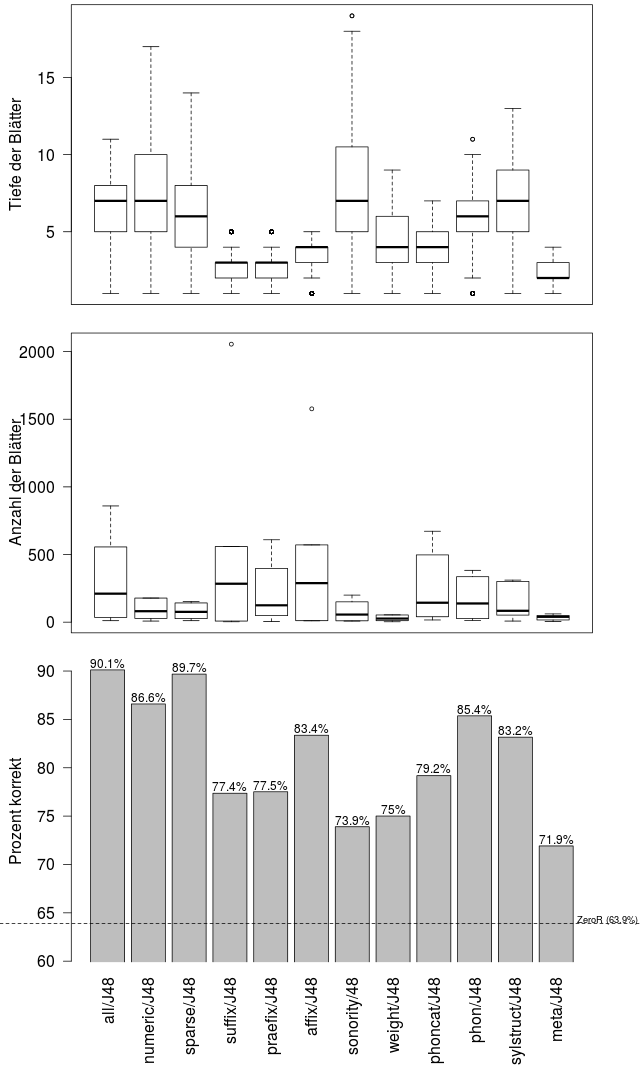
\includegraphics[scale = 0.3]{figures/algorithms/J48.png}} {
            \caption{Metriken zur Analyse der Entscheidungsbäume. Die Tiefe entspricht der Länge der Regel und die Anzahl der Blätter der Anzahl der JRip-Regeln.}
            \label{figure:algorithms_J48}
        }
        \ffigbox{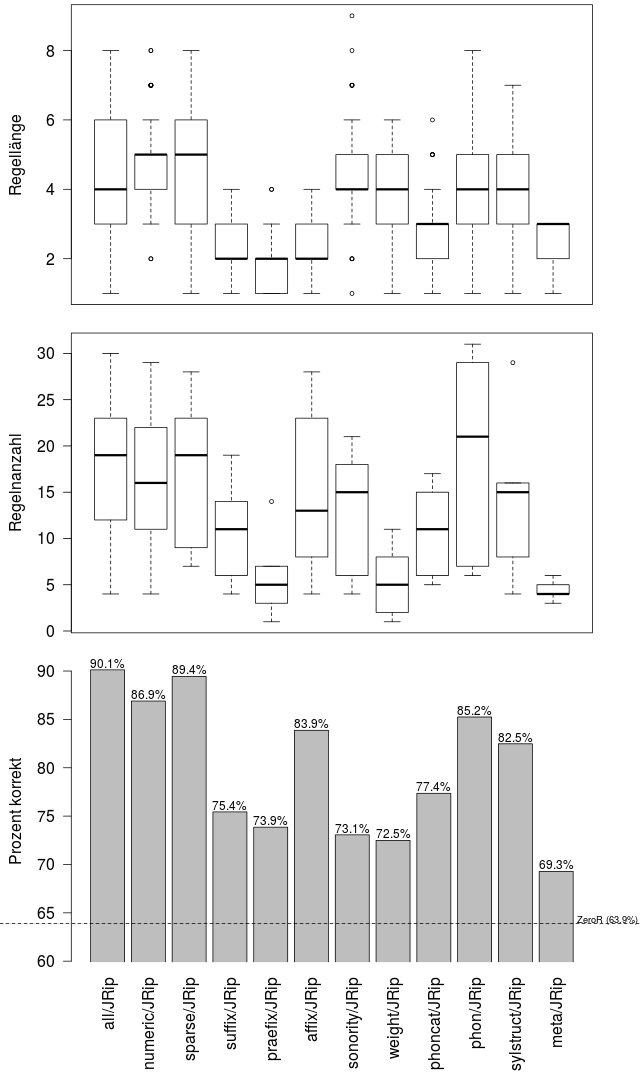
\includegraphics[scale = 0.3]{figures/algorithms/JRip.png}} {
            \caption{Metriken von Analyse der JRip-Regelsätze}
            \label{figure:algorithms_JRip}
        }
    \end{floatrow}
\end{figure}

Ab wann eine Regel \enquote{zu lang} oder ein Regelset \enquote{zu groß} ist, kann man nicht pauschal sagen. Die Anzahl der Regeln wiegt dabei in meinen Augen schwerer als die Länge der Regeln. Die Größe der JRip-Regelsets ist dabei stehts sehr überschaubar, keins hat mehr als etwa 30 Regeln. Die Bäume von J48 hingegen haben oft eine Breite von 500 oder mehr, auch wenn die Mediane um 100-200 herum liegen.
Bei J48 hat das all-Featureset als einziges Modell sowohl eine große Anzahl Blätter als auch gleichzeitig eine recht große Blatttiefe. numeric, sparse, sonority und sylstruct haben zwar sehr Tiefe Blätter, dafür aber nur sehr wenige Knoten. Sie haben jedoch mit die kleinste Merkmalsanzahl (Anhang \ref{attr_counts}), weswegen es nicht verwunderlich ist, dass der Baum statt in die Breite in Tiefe gewachsen ist.
suffix und affix haben beide zwei Ausreißer nach oben in der Anzahl der Blätter. Sie sind neben all und praefix die Featuresets mit den meisten Merkmalen. Diese lassen sich durch die Art und Weise erklären, wie der Baum konstruiert wird. Entscheidet sich beispielsweise der Algorithmus dafür, nach suffix3 zu Unterscheiden, \textit{müssen} alle Werte etwa 90 Ausprägungen (=verschiedene Merkmale) des Features berücksichtigt werden. Geschieht das mehrfach in Folge exponentiert sich die Anzahl der Blätter sehr schnell.

Welche Featuresets sind nun zu bevorzugen bei der Analyse? Das Modell \texttt{all/J48} erzielt zwar die besten Ergebnisse, besitzt jedoch als einziges in Abbildung \ref{figure:algorithms_J48} eine recht große Tiefe und dabei sehr viele Blätter. Es besitzt also beide, eben beschriebenen, nicht wünschenswerte Eigenschaften. Hingegen besitzt sparse/J48 recht wenig Blätter, die zwar recht Tief sind, dafür aber auch das zweitbeste Ergebnis liefert. phon sieht des weiteren vielversprechend aus, Tiefe und Anzahl der Blätter sind in Ordnung, ebenso wie seine Ergebnisse.
Auch hier sticht sonority wieder negativ heraus. Es hat die tiefsten Blätter und das zweitschlechteste Ergebnis, jedoch recht wenige Blätter. Allein scheint dieses Feature sehr schlecht geeignet, den Wortakzent vorherzusagen.  

Bei JRip ist das Problem, dass die Featuresets mit wenigen, kurzen Regeln allesamt schlechte Ergebnisse liefern. Lediglich sieht affix hat sehr kurze Regeln, wenn auch recht viele. Es ist dennoch unter den höheren Featuressets von den Ergebnissen her das schlechteste. Besonders schlecht schneidet wieder sonority mit schlechten Ergebnissen und vielen, langen Regeln ab. Da die Anzahl der Regeln jedoch trotz einer gewissen Varianz stets sehr gering ist, sollte dies kein Argument sein, sie nicht zu untersuchen. Auch die Länge der Regeln ist nicht allzu groß, weswegen es vielversprechend erschient, die mit den besten Erekkungsraten weiter zu untersuchen.

Problematisch bei meinen Metriken ist jedoch, dass der Einfluss der Regeln nicht berücksichtigt wird. So ist es möglich und wahrscheinlich, dass unter vielen langen Regeln auch eine kurze dabei ist, die sehr viele Wörter mit hoher Genauigkeit klassifiziert.
Kritik der Metriken: Einfluss der Regeln nicht berücksichtigt. Viel Totholz, dass den Baum aufbläßt.

%Die Entscheidungsbäume besitzen bei mir eine maximale Tiefe von 10-15, teils bis fast 20, und eine Breite (Anzahl der Blätter) von bis zu 500. Die JRip-Regeln hingegen sind nie länger als 9 Komponenten, meist noch deutlich kürzer, und kein Regelset enthält mehr als ca. 30 Regeln.\\
%So betrachtet sind die JRip-Regeln um ein vielfaches ausdrucksstärker und genereller als die weit ausladenden Entscheidungsbäume von J48. Bei einer Reduktion der Regelanzahl um ca. Faktor 10 sind die Ergebnisse von JRip meist kaum schlechter, in zwei Fällen sogar besser als von J48.

\subsection{Evaluation der Features}

\subsubsection{Manuelle Analyse der Regeln}
Bei der manuellen Durchsicht der Regeln (Auswahl in Anhang \ref{table:jrip_rules_examples}) fallen einige interessante Dinge auf. Recht häufig gibt es im selben Regelset mehrere Regeln, die sich lediglich in einer, oder einigen wenigen, Komponente unterscheiden. Jede Regel dieser \enquote{Regelfamilie} ist für sich genommen recht gut, jedoch ist die Schnittmenge der Wörter, die unter diese Regeln fallen groß. Die Regeln in Abbildung \ref{figure:jrip_tree} klassifizieren zusammen also nicht 1271 Wörter richtig, sondern deutlich weniger.

\begin{figure}
    \tiny
    \centering
    \Tree   [.{comp\_len $\leq$ 1}
                [.{nucleus\_phoncat2 = L}
                    [.{onset\_len0 $\geq$ 1}
                        {pos = V\\\textit{328/8}}
                        {syl\_suffix = ren\\\textit{321/2}}
                        [.{syl\_weight1 = light}
                            [.{prae\_class = ø}
                                {onset\_phoncat3 = C\\\textit{224/40}}
                                [.{syl\_open1 = o}
                                    {sonority\_ratio3 $\leq$ 4\\\textit{34/3}}
                                ]
                            ]
                            {suffix\_phoncat4 = LCKC\\\textit{154.0/27.0}}
                        ] !\qsetw{3cm}
                    ]  !\qsetw{4cm}
                    [.{cv\_ratio1 $\leq$ 0}
                        {syl\_len3 $\geq$ 4\\\textit{167/13}}
                    ]
                    {\qsetw{1cm}suffix3 = sch\\\textit{43/16}}
                ]
            ]
    \caption{Aus sieben ähnlichen JRip-Regeln verschiedener Featuresets generierter Entscheidungsbaum für Viersilbern.\\Die Zahlen unter den Blättern sind die Anzahl an True Positives bzw False Positives. Jeder Ast verbindet zwei Knoten mit einem \enquote{und}.}
    \label{figure:jrip_tree}
    \normalsize
\end{figure}
Eine weiterer Punkt ist, dass viele Regeln unnötig kompliziert sind und teilweise redundant sind. Oft findet man Konstrukte wie \texttt{sonority1 $\geq$ 11 and sonority1 < 11} in den Regeln, da numerische Werte bei JRip nur durch Ungleichungen verglichen werden. Ein weiteres Beispiel ist die Regel \texttt{nucleus\_phoncat0 = K and syl\_phoncat0 = CK}. Ist die Silbe der Gestalt Konsonant (C) - Kurzvokal (K), so ist trivialerweise der Nucleus ein Kurzvokal, da Vokale immer den Nucleus bilden. Extrem häufig beziehen sich Regeln nur auf Nonkomposita (\texttt{comp\_len <= 1}), was für den Linguisten auch wenig interessant ist, da die Betonung von Komposita eigenen Regeln folgen. In sehr vielen Fällen kann man somit noch eine Komponente der Regeln streichen.\\
Mit ein wenig Hintergrundwissen lassen sich die Regeln teils stark vereinfachn. Ein Beispiel ist die Regel \texttt{(nucleus\_phoncat0 = K) and (syl\_weight1 = light) and (sonority0 \textless= 11) and (sonority0 \textgreater= 10) and (syl\_phoncat0 = CKC) and (sonority0 \textgreater= 11)}, die sich mit ein wenig Nachdenken wie folgt schreiben lässt: \texttt{(syl\_phoncat0 = CKC) and sonority0=11 and (syl\_weight1 = light)}. Zudem ergibt sich aus einem Blick in die Tabellen \ref{table:sonority} und \ref{table:phoncats}, dass in einer Silbe der Form CKC eine Sonorität von 11 nur mit bestimmten Klasse von Phonemen möglich ist: Liquid (Sonorität 4) - Approximant (Sonorität 6) - Plosiv/Affrikat/Frikativ (Sonorität 1) bzw. Anfang und Ende vertauscht. Diese anfänglich recht kompliziert erschienende Regel trifft auf ca. 1000 Dreisilber des Testsets zu und klassifiziert rund 80\% davon richtig als paenultimabetont.\\
Vielleicht findet sich diese Regel auch in Regelsets für Wörter mit anderen Silbenzahlen wieder? Woher rühren die 20\% falsch klassifizierten Wörter dieser Regel? Ist die Einteilung der Phonemklassen oder die Sonoritätsskala schuld? Gibt es ähnliche Regeln, die Hinweise zum eigentlichem Kausalzusammenhang liefern können? Da der Zweck dieser Arbeit nicht die Klärung dieser linguistischen Fragen ist, belasse ich es bei diesem Beispiel, das demonstriert welch mächtiges Hilfsmittel die hier angewandten Verfahren sind. In der manuellen Durchsicht der Regeln finden sich noch Unmengen an weiteren Zusammenhängen und Gesetzmäßigkeiten. Es ist jedoch ersichtlich, dass ein gewisses, teils recht umfangreiches Hintergrundwissen notwendig ist, um aus den automatisch generierten Regeln neue Schlüsse ziehen zu können. Maschinelle Verfahren können dabei helfen den Fokus auf die richtigen Aspekte zu lengen, das Schlüsse ziehen nehmen sie uns leider jedoch nicht komplett ab.
\label{rule_simplify}


%%%%%%%%%%%%

%Durch die trennung der Wörter entsprechend ihrer Silbenzahl kann man außerdem beobachten, wie Regeln, die für Wörter mit wenig Silben sehr gut sind, mit steigender Silbenanzahl schlechter werden, man könnte es verrauscht oder gestört nennen. Dies spricht für die Theorie von hierarchischen Regeln, die sich gegenseitig überfahren können.  


%\begin{wraptable}{r}{5cm}
%\centering
%\small
%\caption{Ausdrucksstärkste JRip-Regel bei Dreisilbern:\\(prae\_class = noacc) \\$\implies$ Sekunda wird betont}
%\label{table:noacc_sekunda}
%\begin{tabular}{|cc|}\hline
%{\bf Silben} & {\bf TP/FP}    \\\hline
%2            & 76/0           \\
%3            & 1560/1         \\
%4            & 392/2          \\
%5            & $\approx 98/6$ \\
%6            & 41/5           \\
%7            & -              \\\hline
%\end{tabular}
%\end{wraptable} 

\subsubsection{Einfluss der Features}

\begin{figure}[h]
    \begin{floatrow}
        \ffigbox{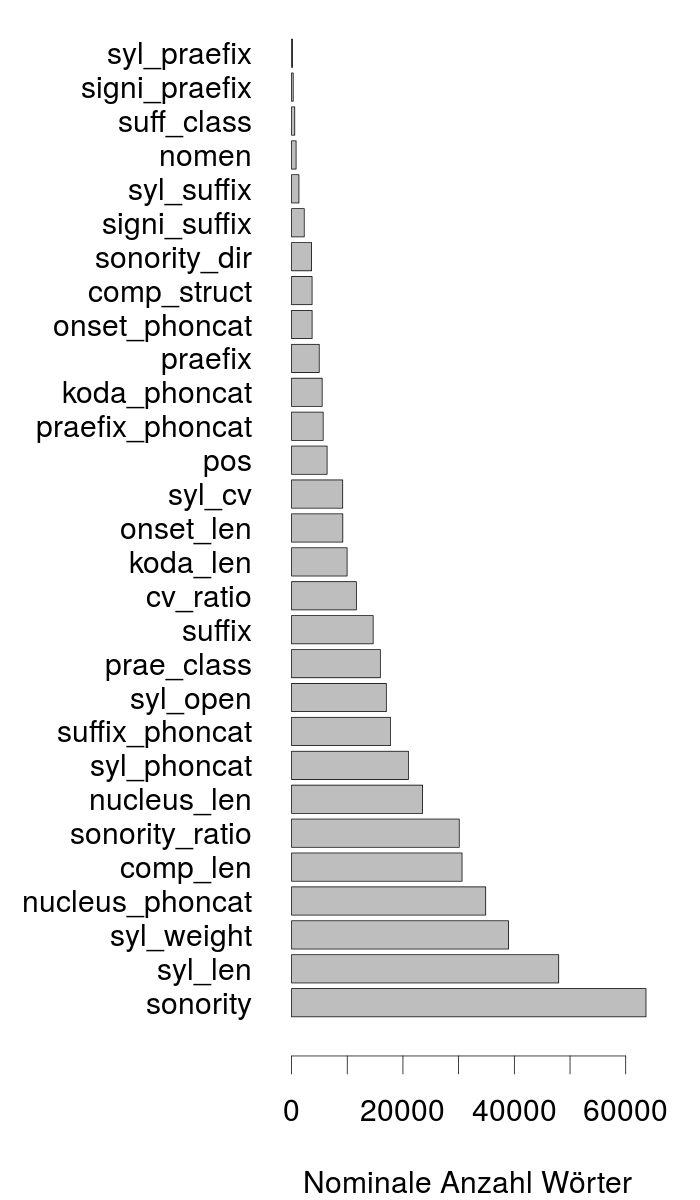
\includegraphics[scale = 0.25]{figures/features/jrip_feature_influence_grouped.png}} {
            \caption{}
            \label{figure:jrip_feature_influence_grouped}
        }
        \ffigbox{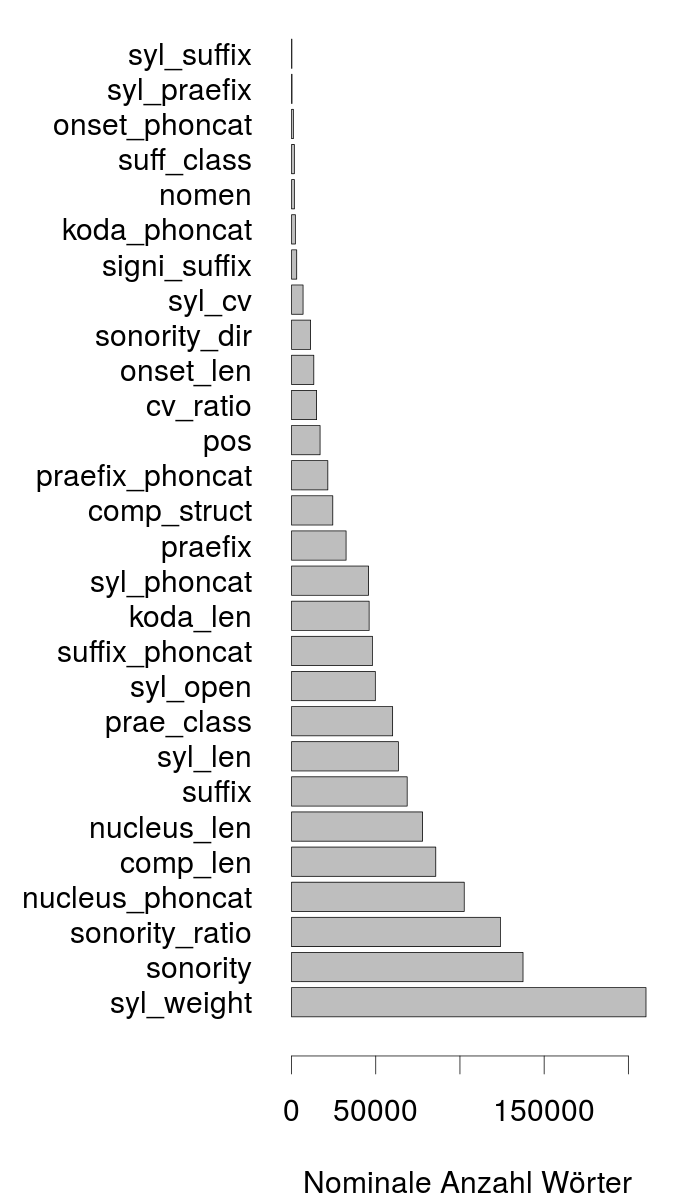
\includegraphics[scale = 0.25]{figures/features/j48_feature_influence_grouped.png}} {
            \caption{}
            \label{figure:j48_feature_influence_grouped}
        }
    \end{floatrow}
\end{figure}

Um den Einfluss der einzelnen Features darstellen zu können, habe ich die Summe der Wörter, 
Die Bedeutung der einzelnen Features für das Gesamtergebnis ist schwierig zu messen. Um dennoch zumindest ein grobes Maß zu erhalten habe ich eine Statistik erstellt, wie viele Wörter von den Regeln erfasst werden, die ein bestimmtes Feature enthalten. Wie bereits erwähnt gibt es bei den Regeln oft ähnliche Varianten, die auf eine große Schnittmenge an selben Wörtern zutreffen. Die Zahlen in Abbildung \label{figure:jrip_feature_influence_grouped} und \label{figure:j48_feature_influence_grouped} sind daher lediglich relativ zueinander zu sehen, die absoluten Zahlen sagen wenig aus. Aus meinen Entscheidungsbäumen habe ich mittels eines kleines R-Skripts Regelsets generiert.

Interessant im Licht der bisherigen Analyse ist, dass die Sonorität und das Silbengewicht die Statistik der JRip-Regeln und Entscheidungsbaum-Regeln anführen. Beim Featureset \texttt{weight} bin ich in Abschnitt \ref{generelles} zu dem Schluss gekommen, das es aufgrund seiner großen Invarianz der Silbenanzahl gegenüber ein recht gut verallgemeinerbares linguistisches Konzept ist. Dies siehe ich durch die häufige Verwendung in einflussreichen Regeln bestätigt. Ähnliches gilt für das grundlegenden Featuresets \texttt{sonority}, das unter Ausschluss anderer Features wenig brauchbar ist, in Kombination aber offensichtlich ein sehr wichtiges Feature darstellt. Die große Bedeutung der Sonorität könnte sich stückweit durch seinen hohen Abstraktionsgrad bei Einbeziehung vieler phonetischer und phonologischer Aspekte sein. Die Sonorität eines Phonems ist eng gekoppelt an seine Phonemklasse und geht dabei weit über die Unterscheidung zwischen Konsonant und Vokal hinaus. Dadurch, dass die Sonorität der Silbe die Summe der Sonorität ihrer Buchstaben ist, sagt die Silbensonorität dabei gleichzeitig auch einiges über die Beschaffenheit der Silbe aus. Zudem ist die Sonorität auch stark mit der Silbenlänge korreliert, die selbst großen Einfluss hat. Je mehr Phoneme die Silbe hat, desto sonoranter kann die Silbe werden. Insgesamt ist die Sonorität ein hervorragendes mittel, viele verschiedene Aspekte einer Silbe numerisch zu repräsentieren.

Mein Feature sonority\_dir, das den Silbensonoritätverlauf über das Wort hinweg repräsentiert scheint hingegen unwichtig zu sein.
Features, die die Suffixe betreffen scheinen wichtiger zu sein als die Präfixe.
Bezüglich der Silbenstruktur ist der Nucleus am wichtigsten, Onset und Koda sind beide recht unwichtig, den Onset jedoch komplett zu ignorieren, wie in der Literatur oft geschieht, sehe ich anhand meiner Daten jedoch nicht gerechtfertigt.



%%%%%%%%%%%%%%%%%
%Welche Features scheinen wichtiger zu sein, welche unwichtiger? Gibt es Features, die immer in Kombination auftreten?
%\subsubsection{Einflussreichste Features}
%\begin{wraptable}{r}{6.5cm}
\tiny
\centering
    \begin{tabular}{|rrr|l|}
    \hline
     $\hat{n}$ & $n$ & $k$ & Feature             \\ \hline
    94                     & 188                & 2                & sonority0        \\
    79,5                   & 159                & 2                & comp\_len        \\
    73                     & 146                & 2                & sonority\_dir    \\
    70                     & 140                & 2                & syl\_len0        \\
    53                     & 106                & 2                & syl\_len1        \\
    49                     & 98                 & 2                & sonority\_ratio0 \\
    46                     & 92                 & 2                & sonority1        \\
    46                     & 92                 & 2                & sonority2        \\
    43                     & 86                 & 2                & sonority3        \\
    41                     & 82                 & 2                & syl\_len2        \\
    36                     & 72                 & 2                & sonority\_ratio1 \\
    34,33                  & 103                & 3                & prae\_class      \\
    33                     & 66                 & 2                & nomen            \\
    32,4                   & 162                & 5                & pos              \\
    32                     & 64                 & 2                & sonority\_ratio2 \\
    30,3                   & 100                & 3,3              & syl\_weight1     \\
    29                     & 58                 & 2                & onset\_len0      \\
    24                     & 48                 & 2                & nucleus\_len1    \\
    23,21                  & 708                & 30,5             & syl\_phoncat1    \\
    23                     & 46                 & 2                & sonority\_ratio3 \\
    23                     & 69                 & 3                & syl\_weight2     \\
    21,03                  & 1912               & 90,9             & suffix3          \\
    20                     & 40                 & 2                & syl\_open2       \\
    20                     & 40                 & 2                & koda\_len1       \\ \hline
    \end{tabular}
    \caption{Normalisierte Häufigkeit der Features in J48-Modellen. Nominalen Häufigkeiten $n$ werden durch den branching factor $k$ zu $\hat{n}=\frac{n}{k}$ normalisiert.}
    \label{table:j48_feature_occurences}
\end{wraptable}
%\begin{table}
    \centering
    \tiny
    \caption{Verwendungshäufigkeit der Features bei allen JRip-Modellen}
    \label{table:jrip_feature_occurences}
    \begin{tabular}{|l|l|} \hline
    Anzahl & Feature \\\hline
     182 & comp\_len         \\
    146  & syl\_weight1      \\
    136  & syl\_len0         \\
    134  & sonority0         \\
    87   & syl\_len1         \\
    81   & prae\_class       \\
    64   & sonority1         \\
    62   & nucleus\_phoncat2 \\
    60   & sonority\_ratio0  \\
    60   & sonority2         \\
    57   & pos               \\
    52   & syl\_weight2      \\
    52   & suff\_class       \\
    48   & syl\_len2         \\
    47   & syl\_phoncat0     \\
    46   & nucleus\_len2     \\
    46   & nucleus\_len1     \\
    45   & onset\_len0       \\
    44   & suffix\_phoncat4  \\
    44   & nucleus\_phoncat1 \\
    43   & sonority3         \\
    35   & syl\_len3         \\
    34   & suffix\_phoncat2  \\
    34   & sonority\_ratio2  \\
    30   & nucleus\_phoncat0 \\
    29   & suffix3           \\
    28   & suffix2           \\
    28   & sonority\_ratio3  \\
    28   & nucleus\_phoncat3 \\
    27   & syl\_open2        \\
    27   & suffix1           \\
    27   & koda\_len2        \\
    27   & cv\_ratio2        \\
    26   & suffix4           \\
    26   & sonority\_ratio1  \\
    26   & nucleus\_len0     \\
    25   & syl\_weight3      \\
    25   & sonority\_dir     \\
    24   & syl\_phoncat3     \\
    23   & syl\_weight0      \\
    23   & syl\_open1        \\
    22   & koda\_len1        \\
    21   & cv\_ratio0        \\
    20   & praefix\_phoncat2 \\
    20   & comp\_struct      \\\hline
    \end{tabular}
\end{table}
%\begin{table}
    \centering
    \small
    \caption{Verwendungshäufigkeit der Features bei allen JRip-Modellen}
    \label{table:jrip_occurences}
    \begin{tabular}{|l|l|}
    \hline
    Jeweils $<$ 10x verwendet	& Jeweils $>$ 25x verwendet \\ \hline
    cv\_ratio4-6	& cv\_ratio2 \\
    syl\_cv4-6	& \\ \hline
    onset\_len1-6	& onset\_len0 \\
    nucleus\_len4-6	& nucleus\_len0-2 \\
    koda\_len3-6	& koda\_len2 \\
    syl\_len5,6 	& syl\_len0-3\\ \hline
    onset\_phoncat0-6 	&  \\
    nucleus\_phoncat4-6 	& nucleus\_phoncat0-3 \\
    koda\_phoncat0,3-6 	&  \\
    syl\_phoncat4-6 	& syl\_phoncat0\\ \hline
    praefix3-5 	& prae\_class \\
    praefix\_phoncat1,3,4,5 	& \\ \hline
    signi\_praefix 	&  \\
    signi\_suffix 	&  \\
    	& suff\_class \\
    	& suffix1-4 \\
    	& suffix\_phoncat2,4\\ \hline
    sonority5,6 	& sonority0-3 \\
    sonority\_ratio4-6 	& sonority\_dir \\
    	& sonority\_ratio0-3\\ \hline
    syl\_open4-6 	& syl\_open2 \\
    syl\_weight5,6 	& syl\_weight1-3\\ \hline
    nomen 	&  \\
    	& comp\_len \\
    	& pos \\ \hline
    \end{tabular}
\end{table}

%\subsubsection{Wenig einflussreiche  Features}
%\begin{wraptable}{r}{5cm}
    \centering
    \tiny
    \caption{Von JRip/J48 auf keinem Trainingsset benutze Features}
    \label{table:unused_features}
    \begin{tabular}{|l|l|}
    \hline
    {\bf J48}	 & {\bf JRip} \\\hline
    cv\_ratio4	&  \\
    cv\_ratio5	&  \\
    cv\_ratio6	 & cv\_ratio6\\\hline
    koda\_len5	 & koda\_len5 \\
    koda\_len6	 & koda\_len6\\\hline
    koda\_phoncat0	&  \\
    koda\_phoncat3	&  \\
    koda\_phoncat4	&  \\
    koda\_phoncat5	 & koda\_phoncat5 \\
    koda\_phoncat6	 & koda\_phoncat6\\\hline
    nucleus\_phoncat5	 & \\\hline
                    	 & nucleus\_phoncat6\\\hline
    onset\_len5	 & onset\_len5 \\
    onset\_len6	 & onset\_len6\\\hline
    onset\_phoncat2	&  \\
    onset\_phoncat3	&  \\
    onset\_phoncat4	&  \\
    onset\_phoncat5	 & onset\_phoncat5 \\
    onset\_phoncat6	 & onset\_phoncat6\\\hline
    sonority6	 & sonority6\\\hline
    sonority\_ratio6	 & sonority\_ratio6\\\hline
    syl\_cv4	&  \\
    syl\_cv6	 & syl\_cv6\\\hline
    	 & syl\_len5 \\
    syl\_len6	 & syl\_len6\\\hline
    syl\_open5	&  \\
    syl\_open6	 & syl\_open6\\\hline
    syl\_phoncat5	 & syl\_phoncat6 \\
    	 & syl\_weight6 \\
    	 & nucleus\_len6 \\\hline
    \end{tabular}
\end{wraptable}
%26 Features wurden über alle 6 Trainingssets hinweg, egal auf welchem Featureset, von keinem einzigen J48 berücksichtigt (Tabelle \ref{table:unused_features}). JRip hat erstaunlicherweise lediglich 19 Features nie berücksichtigt. Bis auf zwei Features, die JRip alleinig nie beachtet hat, decken sich jedoch die Features. Generell sind das Features, die sich auf die hinteren Silben beziehen, die 5, 6, 7. Das ist nicht verwunderlich, da diese Attribute zu kleineren Trainingssets gehören, so dass es schwieriger ist dort Gesetzmä0igkeiten zu erkennen. Ausnahmen hiervon sind koda\_phoncat0 und koda\_phoncat3 und onset\_phoncat2

%\subsubsection{Einflussreichste JRip-Regeln}
%Sämtliche von JRip erzeugte Regeln habe ich mittels eines Shell-Skriptes nach Anzahl der Samples sortiert, auf die diese Regel zutrifft. Die Liste wird von folgender Regel für Dreisilber auf dem \texttt{numeric}-Featureset angeführt:
%\begin{align*}
%\texttt{(comp\_len <= 1) and (sonority\_ratio0 <= 3) and (syl\_len0 <= 3) and}\\
%\texttt{(onset\_len0 >= 1) and (nucleus\_len0 <= 1) and (koda\_len0 <= 0)}\\
%\texttt{=> stress\_class=paenultima}
%\end{align*}
%Dies Regel trifft auf alle 634 Wörter aus dem Testset zu, ohne eine Ausnahme. Das sind immerhin fast 37\% aller Wörter des Testsets mit Paenultima-Betonung. Mit sechs Bedingungen erscheint sie nur mäßig Ausdrucksstark, doch lassen sich aus ihr einige interessante Dinge ableiten. Diese Regel gilt für Nonkomposita (comp\_len <= 1) und betrifft ausschließlich Eigenschaften der ersten Silbe (index 0). Die erste Silbe darf keine Koda haben (koda\_len0 <= 0), muss also offen sein, und der Onset darf nicht leer sein (onset\_len0 >= 1). Der Nucleus des Präfix darf nur aus genau einem Sonoranten bestehen (nucleus <= 1), da jede Silbe einen Nucleus haben muss. Die Silbe darf maximal drei Phoneme enthalten (syl\_len0 <= 3), was bei genau einem Nucleus und ohne Koda eine Onsetlänge von 1 oder 2 ergibt. Die durchschnittliche Sonorität pro Phonem der Silbe muss dabei $\leq3$ sein. Ein Blick in Tabelle \ref{table:sonority} der Sonoritätsklassen zeigt, dass Offene Vokale und Diphtonge mit einer Sonorität von je 10 damit nicht in Wörtern dieser Regel zu finden sein können. 

%(comp_len <= 1) and (cv_ratio0 >= 2) and (sonority0 <= 11) and (syl_len0 <= 3) and (nucleus_len1 >= 2) => stress_class=paenultima (596.0/54.0)

%(comp_len <= 1) and (cv_ratio0 >= 2) and (syl_len0 <= 3) and (sonority_ratio0 <= 3) and (sonority0 >= 11) and (sonority1 >= 12) => stress_class=paenultima (304.0/3.0)


%78\% der Ultimabetonungen bei Dreisilbern werden hiermit erklärt (+6.7\% FP). Der Nucleus der letzten Silbe muss wieder ein Langvokal oder Diphtong sein und mindestens einen Konsonanten enthalten. Hinzu kommt noch, dass die zweite Silbe nur ein oder zwei Phoneme haben darf und die erste Silbe einen Onset haben muss. Diesen beiden sehr guten Regeln gemein ist jedoch die Forderung nach einem Langvokal oder Diphtong in der Ultima. Zwei ähnliche Regeln finden sich auch für Viersilber: Longvokal/Diphtong in der ultima, die Silbe davor maximal zwei Phoneme lang. Die eine Regel fordert dann eine geschlossene 2. Silbe, die andere eine geschlossene letzte Silbe, wobei der Unterschied im Ergebnis minimal ist, also es sich wahrscheinlich lediglich um Koinzidenzien handelt. Festzuhalten ist unzweifelhaft, dass ein Langvokal/Diphtong im Suffix den Akzent anzieht, sofern die Silbe davor recht kurz ist.

%\subsection{Evaluation der Featuresets}

%\begin{center}{
%    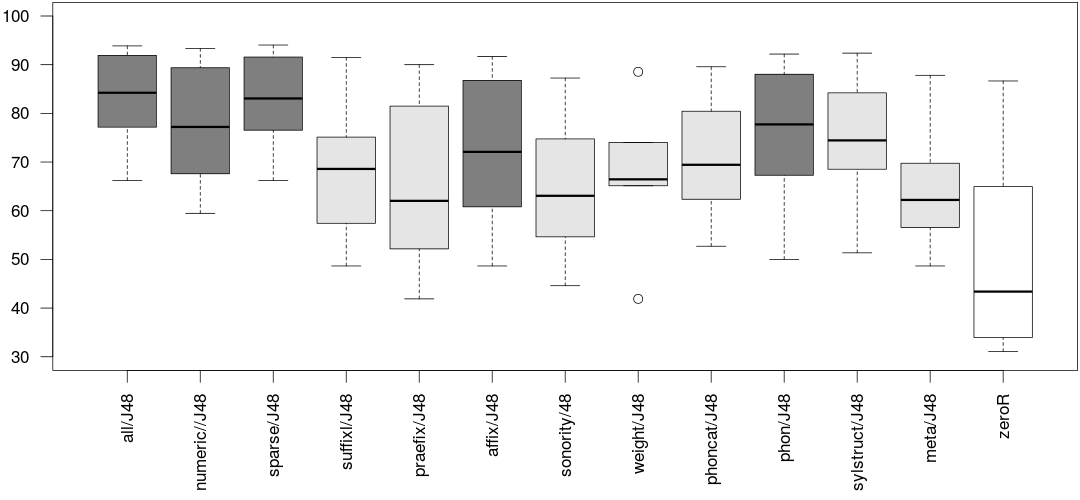
\includegraphics[width=.75\columnwidth]{figures/featuresets/J48.png}
%    \label{figure:featuresets_J48}
%}\end{center}




%\begin{center}{
%    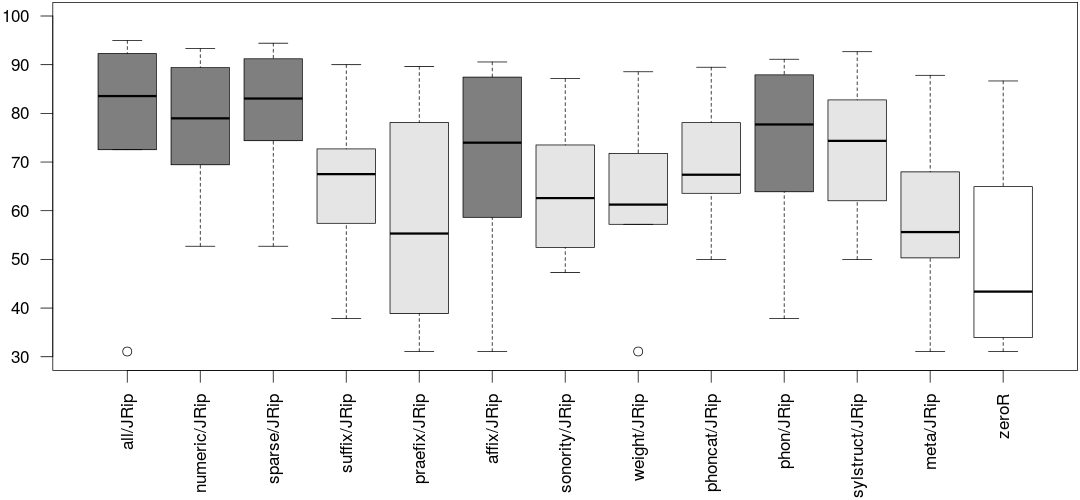
\includegraphics[width=.75\columnwidth]{figures/featuresets/JRip.png}
%    \label{figure:featuresets_JRip}
%}\end{center}

%\begin{center}{
%    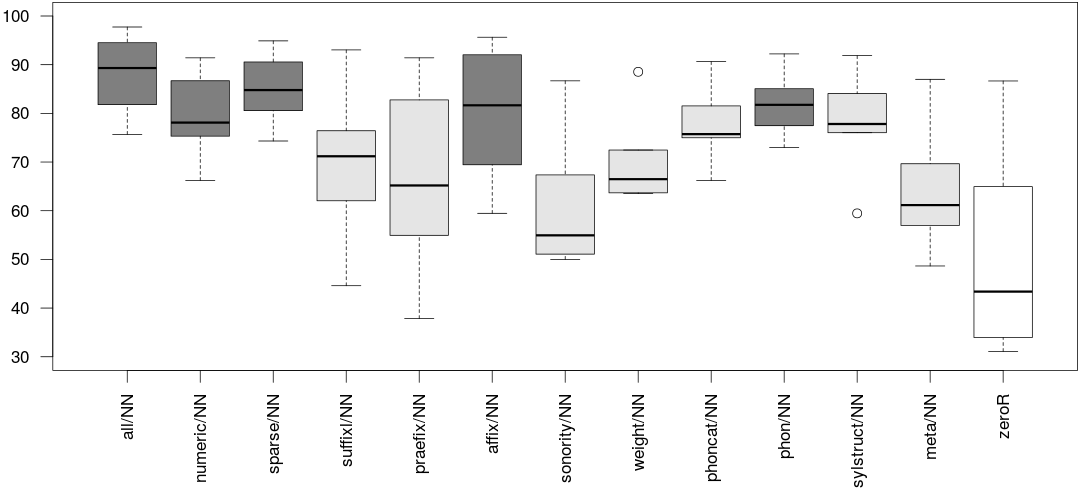
\includegraphics[width=.75\columnwidth]{figures/featuresets/NN.png}
%    \label{figure:featuresets_NN}
%}\end{center}





\subsection{Vergleich zu bisherigen Arbeiten}
%Wie fügt sich meine Arbeit in die Wissenslandschaft ein?

Anzahl Regeln \cite{Rapp1995}

Ergebnisse rein nominal hinter \cite{Hain2004} mit 97.4\%, jedoch hatte er viele Flektionsformen und mehr Daten. Außerdem bei einer 1-to-n Kodierung der Phoneme rund über 400 Inputs (über 40 Phoneme, erste 9 Phoneme).

Daten nicht unbedingt repräsentativ für echten Text, da alle CELEX-Wörter gleichgewichtet. In Realität komische Wörter seltener, daher vmtl besser. Probleme vmtl bei Namen, Fremdwörter sind schwieriger und Komposita.

Nur für Deutsch, Methode lässt sich adaptieren, Ergebnisse nicht. Vielversprehcend jedoch.

Phonemische/Lexikalische Regeln schlecht falls OOV, numerische Werte sehr gut, da immer anwendbar.

Mehr Daten aus wordforms zB wäre sinnvoll, da Erkennungsrate steigt mit Wortanzahl, kein Sättigung \cite[S.~123]{Dou&Bergsma2009}.
Keine linguistischen Regeln, nur statistik, viele Features, mehr Daten. \cite{Dou&Bergsma2009}

%In der Literatur wird häufig Wert darauf gelegt, dass Trainings und Testdaten nicht die gleichen Wortstämme enthalten, damit nicht mit 'sagt' trainiert und mit 'sagen' getestet wird, was möglicherweise die Ergebnisse beeinflussen würde, da die Flektion die betonte Silbe nicht ändert. [ZITAT] Da meine Daten jedoch allesamt Lemmata sind, sind ihre Wortstämme meist verschieden. In meinen Trainings- und Testdaten finden sich insgesamt 2137 Wortstämme, die nicht einzigartig sind, in der Summe sind das 4549 (8,9\%) Wörter.

%%%%%%%%%%%%%%%%%%%%%%%%%%%%%%%%%%%%%%
%%%%%%%%%%%%%%%%%%%%%%%%%%%%%%%%%%%%%%
%%%%%%%%%%%%%%%%%%%%%%%%%%%%%%%%%%%%%%

%In mehr als der Hälfte der Fälle liefern die Neuronalen Netze die besten Ergebnisse, insbesondere auf Featuresets mit vielen verschiednen Werten. J48 ist in den meisten Fällen etwas besser als JRip, große Unterschiede sind recht selten. Die besseren Ergebnisse der NN im Vergleich zu J48, das wiederum leicht besser ist als JRip, lassen sich wahrscheinlich durch die Fähigkeit der Lernalgorithmen erklären, Details zu lernen.


%Paarweise disjunkte Featuresets entsprechend der Betrachutngsebenen         affix   phon    sylstruct   meta            
%(Variante zur differenzierung zwischen Prä und Suffix)                      praefix suffix  phon        sylstruct   meta
%Erweiterung einer sparsamen Grundmenge um hochdimensionale Attribute        all     sparse  numeric             
%Vergleich größter paarweise disjunkter Featuresets                          numeric affix   phoncat     weight          
%Vergleich phonetischer Attribute                                            phoncat weight  sonority                
%Vergleich kleinster paarweise disjunkter Featuresets                        praefix suffix  phoncat     weight      sonority    sylstruct   meta
